\section{Integrated Results and Discussion}
\label{sec:discussion}

\subsection{How the analyses should be compared}

The analyses in this report address related but distinct questions.  The
reference-study reproduction examines whether the published diagnostic and
prognostic procedures can be reconstructed using the available Surveillance,
Epidemiology, and End Results (SEER) registry extract.  External validation asks
whether the resulting reference models retain predictive value when applied
unchanged to patients from University Hospital Erlangen
(\emph{Universit{\"a}tsklinikum Erlangen}, abbreviated as UK Erlangen).  The
transformation analyses examine which predictive and structural properties are
retained in TabPFN representations and synthetic datasets.  The matched model
benchmark compares algorithms trained and evaluated on the same real-patient
partitions.  Finally, the augmentation analysis asks whether adding synthetic
records improves each model relative to its own real-only result.

These results should not be combined into a single ranking.  A numerical model
comparison is most informative when the models use the same outcome, training
patients, test patients, preprocessing and performance measure.  Results from
the reference reproduction, transformed datasets and matched benchmark differ
in one or more of these respects.  They can be interpreted together, but their
performance values are not directly interchangeable.

\begin{table}[htbp]
\centering\scriptsize
\setlength{\tabcolsep}{3pt}
\caption{Purpose and main limitation of each analysis used in this integrated
discussion.}
\label{tab:discussion:evidence-hierarchy}
\begin{tabularx}{\linewidth}{@{}>{\RaggedRight\arraybackslash}p{2.55cm}>{\RaggedRight\arraybackslash}p{3.0cm}>{\RaggedRight\arraybackslash}p{3.35cm}Y@{}}
\toprule
Analysis & Evaluation data & What the analysis can show & Main limitation \\
\midrule
\csname @@input\endcsname{tables/integrated_discussion/evidence_hierarchy_rows.tex}
\bottomrule
\end{tabularx}
\end{table}

Table~\ref{tab:discussion:evidence-hierarchy} separates the five types of
evidence used below.  A successful reproduction shows that a published workflow
can be reconstructed, but does not show how well it will perform in new
patients.  A transformation may retain predictive information without
improving a downstream model.  Synthetic records may resemble the real data in
their overall distributions without adding independent clinical information.
Independent hospital patients provide stronger evidence of transportability,
but the UK Erlangen sample is too small for precise estimates or reliable
subgroup conclusions.  These distinctions guide the integrated interpretation.

\subsection{Integrated diagnostic findings}
\label{sec:discussion:diagnostic}

The diagnostic reproduction found substantial predictive signal in the
available SEER cohort.  When each model was fitted and evaluated in the complete
2,672-patient development cohort, the area under the receiver operating
characteristic curve (ROC AUC) was 0.8795 for the fixed 5-variable nomogram,
0.8947 for the 6-variable specification described in the reference-paper text,
0.9028 for the 8-variable data-driven model and 0.7628 for the American Joint
Committee on Cancer (AJCC) T/N-stage comparator.  The reference study reported
an AUC of 0.877 in its SEER development cohort and 0.893 in its external
hospital cohort.  The similar magnitudes support the reconstruction of the
published approach, but the present within-cohort values are not estimates of
performance in new patients and were obtained from a different SEER release.

The UK Erlangen analysis provides independent evaluation of the unchanged
reference models.  In the common 29-patient complete-case set, the 5-variable
nomogram achieved an AUC of 0.934 (95\% confidence interval 0.809--1.000), the
8-variable model achieved 0.942 (0.837--1.000), and the T/N-stage comparator
achieved 0.739 (0.521--0.927).  These findings show that the multivariable
models retained diagnostic ranking ability in this hospital cohort.  However,
only 10 patients had the diagnostic outcome, producing wide intervals and
unstable calibration and decision-curve estimates.  The analysis therefore
supports preliminary transportability, not a precise ranking of the models or
a validated clinical threshold.

The matched real-patient benchmark provides the most reliable comparison of
model families within SEER (Table~\ref{tab:discussion:diagnostic}).  TabPFN-3,
TabICLv2 and TabDPT formed a narrow leading group, with real-only ROC AUC values
of 0.902--0.903.  Relative to logistic regression, their paired AUC differences
were 0.0088 (95\% interval 0.0034--0.0145), 0.0075 (0.0021--0.0132) and
0.0074 (0.0016--0.0133), respectively.  TabPFN-3 and TabICLv2 also improved
average precision by approximately 0.03 and reduced Brier score by 0.0043.
TabDPT reduced Brier score by 0.0033, while its average-precision interval
included zero.  The differences are small, but they consistently favour the
three foundation models for diagnostic ranking under this internal evaluation
design.

\begin{table}[htbp]
\centering\scriptsize
\setlength{\tabcolsep}{2.3pt}
\caption{Integrated diagnostic results under the matched clinical-variable
design.  AUC, average precision (AP) and Brier score are real-only estimates.
Paired changes compare maximum augmentation (\texttt{+15K}) with the same model
trained on real data alone (\texttt{+0}); positive changes favour augmentation.
Intervals are pointwise 95\% patient-bootstrap intervals conditional on the
fitted models.}
\label{tab:discussion:diagnostic}
\begin{tabularx}{\linewidth}{@{}>{\RaggedRight\arraybackslash}p{2.15cm}rrrYY@{}}
\toprule
Model & AUC & AP & Brier & $\Delta$ AUC at +15K &
Brier improvement at +15K \\
\midrule
\csname @@input\endcsname{tables/integrated_discussion/diagnostic_synthesis_rows.tex}
\bottomrule
\end{tabularx}
\end{table}

The clinical multilayer perceptron (MLP) reached an AUC of 0.897, an AP of 0.652
and a Brier score of 0.088.  Its paired AUC and AP differences from logistic
regression included zero.  The MLP adds nonlinear modelling capacity without
foundation-model pretraining, so this result shows that nonlinearity alone did
not reproduce the small diagnostic advantage of the foundation models under the
tested protocol.  It does not prove that pretraining caused the difference,
because the architectures, regularization, optimization and model-specific
assumptions also differ.

Synthetic augmentation changed performance selectively.  XGBoost, which had
the lowest real-only diagnostic AUC, improved from 0.883 to 0.895 and reduced
its Brier score from 0.096 to 0.090 at \texttt{+15K}; both paired intervals
excluded zero.  Logistic regression and the MLP showed no clear change.
TabPFN-3 had small AUC and Brier-score deteriorations, TabICLv2 had a small
Brier-score deterioration, and TabDPT's maximum-size changes were inconclusive.
Synthetic augmentation therefore helped one diagnostic estimator but did not
act as a general increase in effective sample size.

\subsection{Integrated prognostic findings}
\label{sec:discussion:prognostic}

The reproduced 5-variable prognostic model also retained survival ordering in
the held-out 30\% SEER subset.  Its time-dependent AUCs were 0.886, 0.873 and
0.844 at 12, 24 and 36 months.  These results come from one 70/30 split and
should not be compared directly with the matched benchmark, which averages
five held-out splits and uses additional measures such as Uno's concordance
index and the integrated Brier score (IBS).

In the independent UK Erlangen cohort, the primary prognostic nomogram achieved
a Harrell concordance index of 0.833 (95\% confidence interval 0.625--1.000) in
all 11 liver-metastasis-positive patients.  In the 10-patient set shared with
the T/N-stage model, the corresponding values were 0.824 for the nomogram and
0.676 for T/N stage.  Nomogram AUC estimates were 0.954, 0.936 and 0.833 at 12,
24 and 36 months, but every interval was wide.  These results are consistent
with retained prognostic ranking in independent patients, while remaining too
imprecise to establish external performance with confidence.

Under the matched SEER design, discrimination was tightly clustered
(Table~\ref{tab:discussion:prognostic}).  TabPFN landmark had the highest
real-only Uno concordance point estimate at 0.717, followed by random survival
forest at 0.712 and Cox elastic net at 0.711.  None of the planned paired
comparisons established a concordance advantage over its conventional
reference.  Random survival forest provided the best probability-error result:
its IBS of 0.153 improved on Cox elastic net by 0.0071 (95\% interval
0.0012--0.0128).  It also had the smallest mean absolute Kaplan--Meier (KM)
calibration gap, 0.044.  Thus an established survival model gave the strongest
probability-accuracy result, while no prognostic foundation-model advantage was
demonstrated.

\begin{table}[htbp]
\centering\scriptsize
\setlength{\tabcolsep}{2.2pt}
\caption{Integrated prognostic results under the matched clinical-variable
design.  Uno's concordance index (Uno C), IBS and the mean absolute KM
calibration gap are real-only estimates.  Paired changes compare
\texttt{+15K} with \texttt{+0}; positive changes favour augmentation.  The KM
gap averages the 15 estimable split--horizon combinations, each based on three
risk groups.}
\label{tab:discussion:prognostic}
\begin{tabularx}{\linewidth}{@{}>{\RaggedRight\arraybackslash}p{2.35cm}rrrYY@{}}
\toprule
Model & Uno C & IBS & KM gap & $\Delta$ Uno C at +15K &
IBS improvement at +15K \\
\midrule
\csname @@input\endcsname{tables/integrated_discussion/prognostic_synthesis_rows.tex}
\bottomrule
\end{tabularx}
\end{table}

The clinical prognostic MLP showed no general advantage over the matched Cox or
random-survival-forest models.  Its real-only Uno concordance was 0.709 and its
IBS was 0.162.  Augmentation did not reverse this result.  At \texttt{+15K},
Cox elastic net lost 0.0250 in Uno concordance and worsened by 0.0214 on the
favourably oriented IBS scale.  The MLP's concordance change was inconclusive,
but its IBS worsened at every augmentation size and by 0.0136 at
\texttt{+15K}.  Changes for random survival forest, TabPFN landmark and
SurvivalPFN included zero for both main paired outcomes at the maximum size.

The prognostic training partitions contained a mean of only 323 real patients.
At \texttt{+15K}, synthetic records accounted for 97.9\% of the combined
training rows.  This dominance of the generated distribution occurred together
with outcome shifts, absent grade-4 support and small inconsistencies between
linked variables.  These observations are compatible with the lack of
prognostic benefit, but they do not identify a single causal explanation.

\begin{figure}[htbp]
\centering
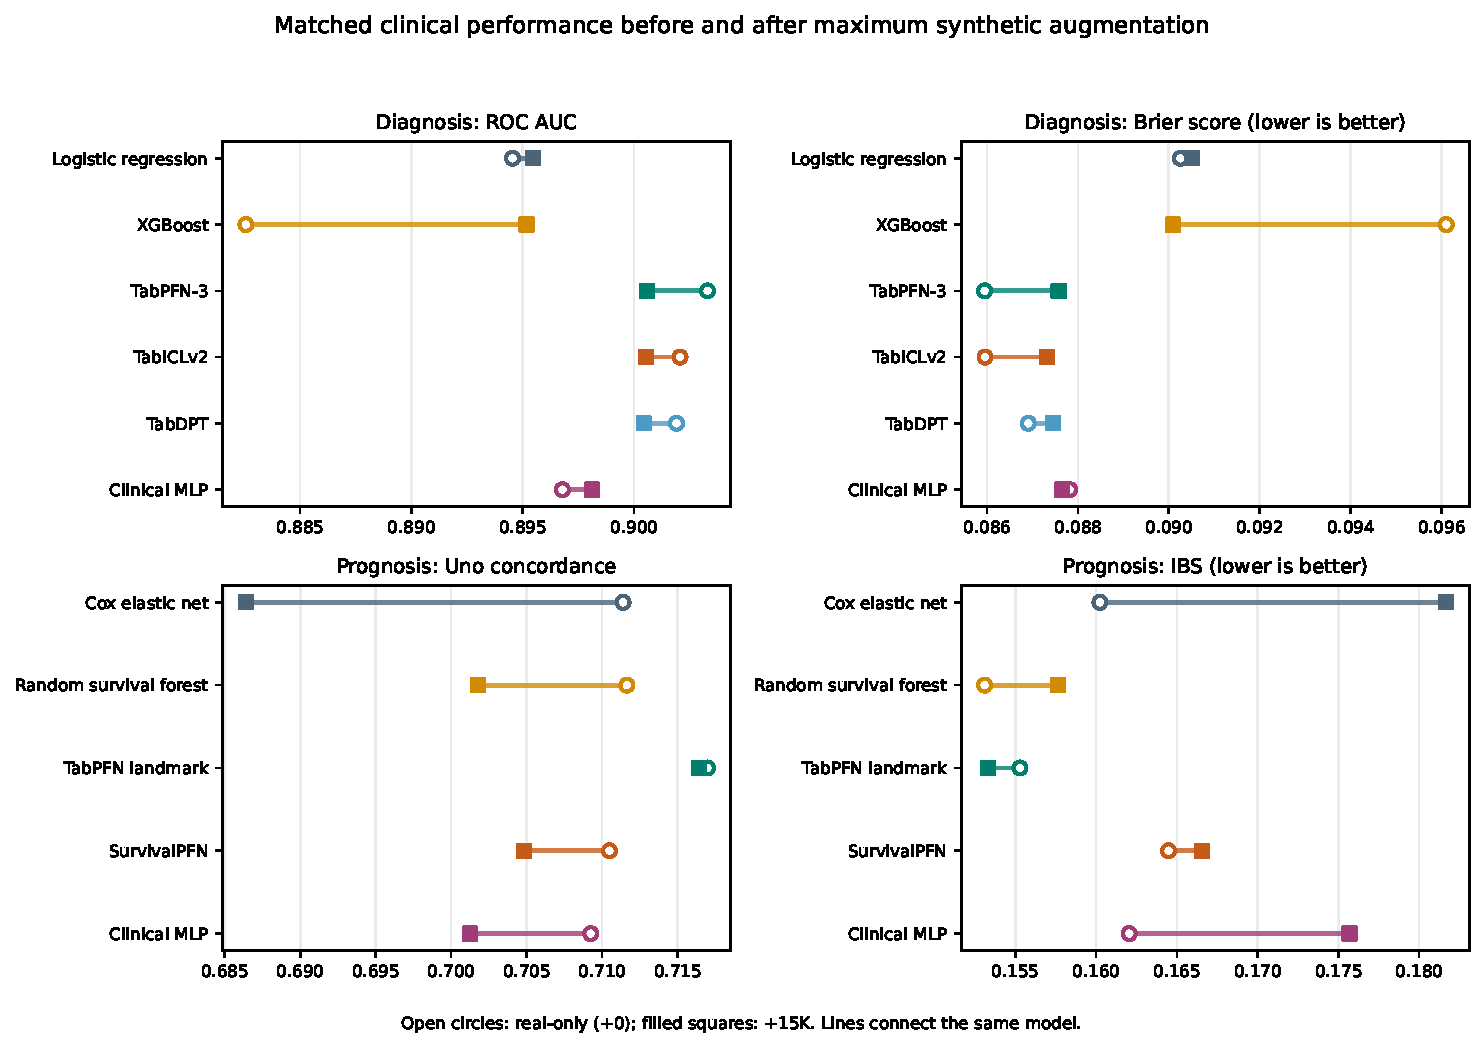
\includegraphics[width=0.98\linewidth]{integrated_discussion/integrated_matched_clinical_landscape.pdf}
\caption{Matched real-only performance (open circles) and performance after
adding 15,000 training-partition-specific synthetic records (filled squares).
Lines connect results for the same model and show direction, not statistical
significance.  Movement to the right is favourable for AUC and Uno concordance;
movement to the left is favourable for Brier score and IBS.  Results from the
reference reproduction and full-cohort transformations are excluded because
they use different evaluation designs.}
\label{fig:discussion:clinical-landscape}
\end{figure}

\subsection{What the transformations preserved}
\label{sec:discussion:transformations}

The TabPFN embeddings retained substantial predictive information.  A
regularized diagnostic model trained on the 512-dimensional representation
reached an AUC of 0.900.  The prognostic representation produced AUCs of 0.861,
0.858 and 0.843 at 12, 24 and 36 months, close to the corresponding clinical-
model values of 0.886, 0.873 and 0.844.  Local-neighbour preservation was high:
trustworthiness and continuity were approximately 0.95 for diagnosis and
0.84--0.88 for prognosis.  Correlations between the complete clinical and
embedding distance matrices were more moderate, ranging from 0.400 to 0.558.
The embeddings therefore retained local patient relationships more strongly
than the overall geometry of the clinical feature space.

These representation results remain exploratory because the embeddings were
created from the complete cohort before the later training and test partitions
were defined, and supervised outcomes were used during their construction.
Resampling only the prediction model fitted on those representations does not
show how an embedding generated exclusively from training patients would
perform in unseen patients.

\begin{table}[htbp]
\centering\scriptsize
\setlength{\tabcolsep}{3pt}
\caption{Integrated interpretation of the TabPFN transformations and the
training-partition-specific augmentation experiment.  Performance values remain
within their original evaluation designs and should not be treated as a common
model ranking.}
\label{tab:discussion:transformations}
\begin{tabularx}{\linewidth}{@{}>{\RaggedRight\arraybackslash}p{2.35cm}>{\RaggedRight\arraybackslash}p{3.15cm}>{\RaggedRight\arraybackslash}p{3.0cm}>{\RaggedRight\arraybackslash}p{3.0cm}Y@{}}
\toprule
Analysis & Predictive result & Structural result & Evaluation design & Conclusion \\
\midrule
\csname @@input\endcsname{tables/integrated_discussion/transformation_synthesis_rows.tex}
\bottomrule
\end{tabularx}
\end{table}

The synthetic datasets generated from the complete SEER cohorts reproduced many
individual-variable distributions and allowed the diagnostic and prognostic
pipelines to run.  However, a classifier could distinguish real from synthetic
records; grade 4 was absent; survival distributions shifted; and several
relationships between variables were incompletely preserved.  Because the
generator learned from all observed patients and evaluation was performed on
generated data or with unequal real-to-synthetic directions, these experiments
describe fidelity and pipeline behaviour rather than performance in unseen real
patients.

The augmentation experiment provides the more direct test of practical utility.
For every evaluation partition, synthetic records were generated using only the
real training patients, and performance was measured only in the held-out real
patients.  Its mixed results show why distributional similarity and predictive
utility are different properties.  Small Jensen--Shannon or standardized
Wasserstein distances did not guarantee improved prediction, while XGBoost
benefited despite known differences in grade support and outcome prevalence.
Utility depended on the task, model, real sample size and proportion of
synthetic training records.

\subsection{What the model comparisons suggest}

For diagnosis, all three pretrained tabular models showed small matched
improvements over logistic regression, whereas the clinical MLP did not.  This
pattern is compatible with useful information from pretraining or
context-dependent inference, but the study was not designed to isolate the
effect of pretraining.  The MLP architecture, optimization procedure and
regularization differed from those of the foundation models, and only one
prespecified MLP design was tested.  The defensible conclusion is therefore
empirical: under the tested protocol, adding generic nonlinear capacity did not
match the strongest diagnostic results.

Prognosis was more difficult.  It combined censoring, multiple time horizons
and a substantially smaller sample.  The models also represented survival in
different ways: Cox regression estimated proportional hazards, random survival
forest modelled survival nonlinearly, TabPFN landmark used separate binary
predictions at each horizon, and SurvivalPFN used survival-specific pretraining.
These differences make small point-estimate gaps difficult to interpret as a
general advantage of one model family.  The results favour larger, event-rich
cohorts and survival-specific model development rather than assuming that gains
in binary diagnosis will transfer to prognosis.

\subsection{Calibration, subgroup support and clinical meaning}

Discrimination does not describe probability accuracy or clinical usefulness
on its own.  In the real-only diagnostic benchmark, TabDPT had a calibration
slope closest to one at 1.001, followed by logistic regression at 0.960.
TabPFN-3, TabICLv2 and the MLP had slopes of 0.899, 0.910 and 0.893.
Augmentation improved XGBoost's slope from 0.731 to 0.878 but moved TabPFN-3 and
TabICLv2 farther from one.  In prognosis, random survival forest had the lowest
IBS and KM calibration gap despite not having the highest concordance.  The
model favoured by discrimination was therefore not always the model favoured by
calibration or probability error.

Decision-curve results describe net benefit across selected risk thresholds,
but they do not identify a clinically validated threshold or demonstrate
patient benefit.  Rare-group support is an additional limitation.  Diagnostic
grade-4 performance could be estimated in only 44 of 1,100 fold-level
model conditions, although combining predictions across folds allowed all 220
repeat-level conditions to be summarized.  No prognostic split supported a
grade-4 estimate.  Grade 4 was absent from every synthetic pool and became
progressively diluted as the synthetic fraction increased.  The report cannot
therefore support conclusions about equal performance or benefit in this rare
group.

\subsection{Answers to the project objectives}
\label{sec:discussion:objectives}

Table~\ref{tab:discussion:objectives} summarizes the findings for the nine
objectives defined in Section~\ref{sec:introduction:objectives}.  The data,
reproduction and dataset-construction objectives were completed.  The empirical
objectives produced qualified findings: predictive information was retained
after transformation, but the embedding and complete-synthetic-dataset results
have design limitations; three diagnostic foundation models showed modest
matched gains; the tested MLP did not show a general advantage; and synthetic
augmentation helped diagnostic XGBoost without improving prognosis.

\begin{table}[H]
\centering\scriptsize
\setlength{\tabcolsep}{3pt}
\caption{Integrated answers to the nine project objectives.}
\label{tab:discussion:objectives}
\begin{tabularx}{\linewidth}{@{}>{\RaggedRight\arraybackslash}p{0.45cm}>{\RaggedRight\arraybackslash}p{2.45cm}Y>{\RaggedRight\arraybackslash}p{3.05cm}@{}}
\toprule
ID & Objective & Main finding & Interpretation and limitation \\
\midrule
\csname @@input\endcsname{tables/integrated_discussion/objective_synthesis_rows.tex}
\bottomrule
\end{tabularx}
\end{table}

\subsection{Overall interpretation}

The project completed an end-to-end analysis from SEER cohort construction to
reference-model reproduction, external evaluation, tabular foundation models,
learned representations, synthetic data, nonlinear MLPs and synthetic-data
augmentation.  The clearest model-comparison result was a small diagnostic
advantage for three tabular foundation models under matched real-patient
validation.  The clearest augmentation result was more specific: synthetic
records improved diagnostic XGBoost, but did not provide a general benefit and
slightly worsened some already strong models.  No corresponding foundation-model,
MLP or augmentation benefit was demonstrated for prognosis.

The overall findings do not support a simple conclusion that more complex
models or more generated data necessarily improve clinical prediction.
Performance depended on the task, evaluation design, estimator, real sample
size and which relationships were preserved by the transformation.  Future
work should generate representations separately within training partitions,
preserve rare clinical categories explicitly, evaluate synthetic data in larger
independent cohorts and develop survival-specific foundation models using more
event-rich data.  The present results remain research findings and do not
establish readiness for clinical deployment.  The next section consolidates
the study's remaining limitations.

\FloatBarrier
